\documentclass{article}
\usepackage[utf8]{inputenc}

\title{\vspace{-4cm} Mapper \\ \vspace{0.2cm} \large Topological Data Analysis}
\author{Jana Řežábková, Jan Joneš}
\date{15. 1. 2021}

\usepackage{amsmath}
\usepackage{amssymb}
\usepackage{hyperref}
\usepackage{graphicx}

\graphicspath{{./figures/}}

\begin{document}

\maketitle

\section{Introduction}

Visualization of high-dimensional data is hard.
In the field of topological data analysis, Mapper~\cite{mapper} is one popular method used for data visualization.

In this report we provide a simple yet fast implementation of Mapper in Python that works on 3D points.

\section{Algorithm}

Input to the Mapper algorithm is finite point cloud $X \subset \mathbb{R}^3$.
We demonstrate how the algorithm works on an example of torus whose points are shown in Figure~\ref{fig:torus-points}.

\begin{figure}[ht]
    \centering
    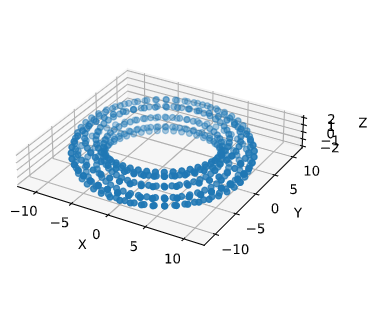
\includegraphics[width=0.7\columnwidth]{torus-point-cloud}
    \caption{Point cloud of torus example.}
    \label{fig:torus-points}
\end{figure}

The algorithm first applies filter function $f: X \to I$ where $I \subseteq \mathbb{R}$, mapping each point to real space.
Filter function can be arbitrary and its choice usually depends on the input data.
Commonly used filter functions are
\begin{itemize}
    \item specific coordinate, e.g., y coordinate $f((x, y, z)) = y$,
    \item distance from point $\mathbf{p}$, i.e., $f(\mathbf{x}) = \lVert \mathbf{x} - \mathbf{p} \rVert_2$, where origin is usually used as $\mathbf{p}$.
\end{itemize}
Applying filter function to our torus example is demonstrated in Figure~\ref{fig:torus-filter}.

\begin{figure}[ht]
    \centering
    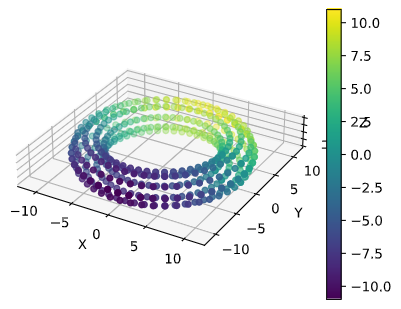
\includegraphics[width=0.4\columnwidth]{torus-y-coor}
    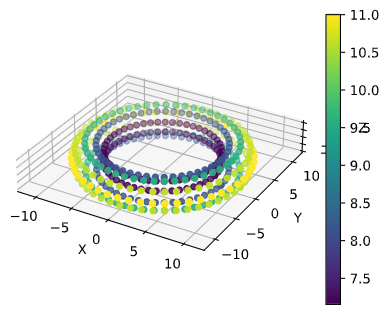
\includegraphics[width=0.4\columnwidth]{torus-distance-from-origin}
    \caption{Different filter functions applied to our torus example.
        On the left, y coordinate; on the right, distance from origin.
        Value of the filter function is illustrated using color range.}
    \label{fig:torus-filter}
\end{figure}

We continue by splitting the interval into overlapping bins.
Formally, we take $\mathcal{U} = \{ U_\alpha \}_{\alpha \in A}$ finite covering of $I$.
Usually, uniform covering is used.
Then, it is enough to specify number of bins and ratio of overlap.

\begin{figure}[ht]
    \centering
    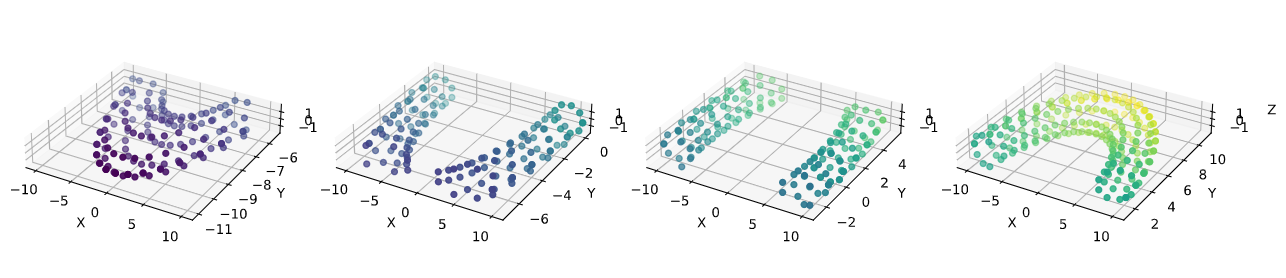
\includegraphics[width=0.9\columnwidth]{torus-partition-4-25}
    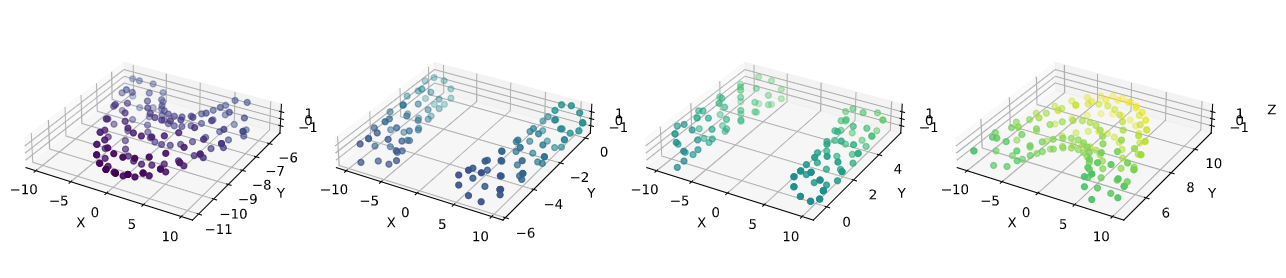
\includegraphics[width=0.9\columnwidth]{torus-partition-4-05}
    \caption{Different coverings used in our torus example.
        We use 4 bins with 25~\% overlap in the top row and 5~\% overlap in the bottom row.}
    \label{fig:torus-cover}
\end{figure}

\bibliographystyle{IEEEtran}
\bibliography{bibliography}

\end{document}
